\section{Relative positioning}
A relative position is a position that is relative to something absolute. A technique called dead reckoning is very useful in situations where one have to move away from a absolute position, therefore won't be able to get another for a while. Such as in a network game or outside hiking with no GPS. To use dead reckoning you need keep track of things can that help you navigate such as. 
\begin{itemize}
\item Direction of travel.
\item Pace.
\item Time of walking.
\item Landmarks.
\end{itemize}
When a trip starts we know we are at a absolute position the base camp and we want to reach the destination as shown in figure \ref{fig:deadrecdrawing}. We use our pace, compas and the landmarks to navigate to the destination.
\begin{figure}[H]
	\centering
	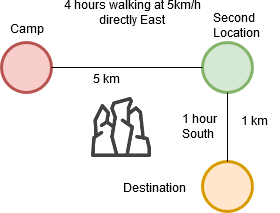
\includegraphics[width=0.4\linewidth]{positioning/positioning/deadRecDrawing}
	\caption{A hiking trip with navigation using dead reckoning.}
	\label{fig:deadrecdrawing}
\end{figure}
But dead reckoning suffers from errors that are cumulative, for example, if the first part of the example had ended up being 8 km instead of 5 then even if the second part goes according to plan, you are still going to end up in the wrong place. A way to solve this problem is to find your absolute location with bearings from time to time as that will reset the drift in regard to possible errors.
\section{Dead recking in network games}
Dead recking is not only used at sea or to navigate the land, but also in distributed virtual environments. When people a cross the planet play networked games they are sometimes placed between very far between each other. In the Pentel and Wolf paper\footnote{\cite{Pantel2002}} they explore different dead reckoning schems in different game types such as a Sport game and 3D action game. There were 8 prediction schemes, 4 position, 3 input and one no prediction scheme. As shown in Figure \ref{fig:wolfpeperimage} \footnote{\cite{Pantel2002} p81} the Prediction 1 which predicts the position by assuming a constant velocity is a yield the best result.
\begin{figure}[H]
	\centering
	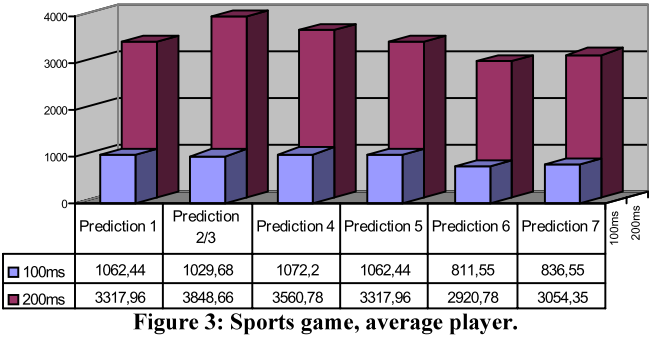
\includegraphics[width=0.5\linewidth]{positioning/positioning/wolfpeperImage}
	\caption{Prediction 1 was best in a sports game}
	\label{fig:wolfpeperimage}
\end{figure}
They conclude that the different schemes they looked at was useful for network games. But they could not reduce the latency directly, but the impacted of it could be.